\documentclass[]{standalone}
\usepackage{tikz}
\usepackage{siunitx}
\usetikzlibrary{patterns,arrows}
\definecolor{silver}{rgb}{0.75, 0.75, 0.75}

\begin{document}
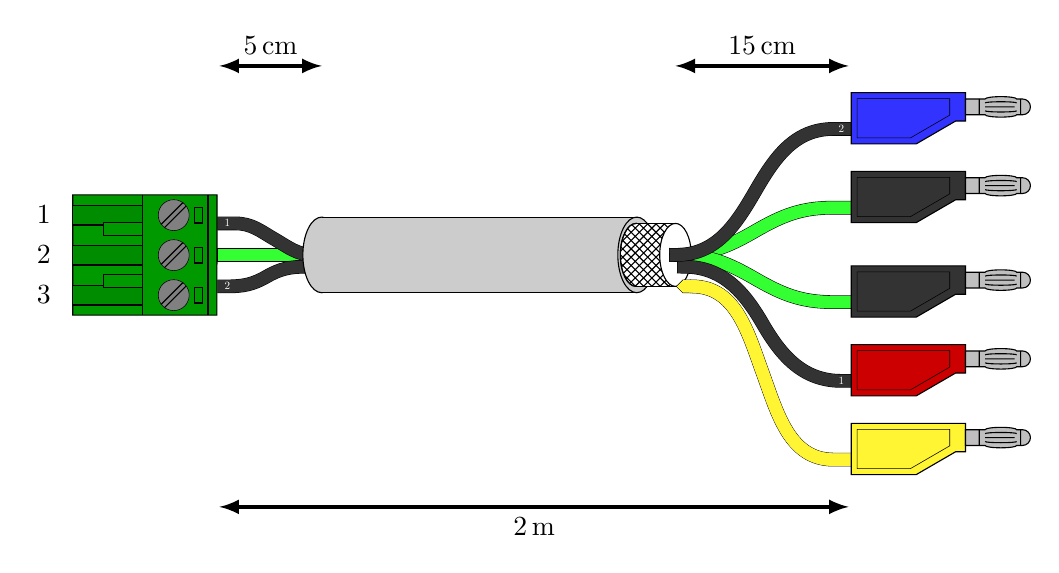
\begin{tikzpicture}[x=1mm, y=1mm, scale=2, transform shape]
    \def\cylinder#1#2#3#4#5{
        % #1 diameter
        % #2 length
        % #3 color
        % #4 pattern
        % #5 label
        \draw[fill=#3, #5]%
            (-#2,0) ellipse (#1/4 and #1/2)%
        ;%
        \draw[#4, #5]%
            (-#2,0) ellipse (#1/4 and #1/2)%
        ;%
        \fill[#3]%
            (-#2,#1/2) rectangle (0,-#1/2)%
        ;% background
        \fill[#4]%
            (-#2,#1/2) rectangle (0,-#1/2)%
        ;%
        \draw[fill=#3, #5]%
            (0,0) ellipse (#1/4 and #1/2)%
        ;%
        \draw[#5]%
            (0,#1/2) --    +(-#2,0)%
            (0,-#1/2) -- +(-#2,0)%
        ;%
    }

    \def\wire#1#2#3#4#5{
        % #1 color
        % #2 length
        % #3 height
        % #4 x shift
        % #5 angle
        % If we must have rounded caps, check out:
        % https://tex.stackexchange.com/questions/21392/rounded-ends-with-tikz
        \draw[very thin, double distance = 0.8mm*2, double=#1, line cap=rect]%
            (0mm,0mm) to[out=0, in=#5-180] ++(#2/2,#3/2) to[out=#5, in=180] ++(#2/2,#3/2) -- ++(#4,0) -- ++(0.2mm,0)%
        ;
    }

    \def\wireWithTip#1#2#3#4#5{
        % #1 color
        % #2 length
        % #3 height
        % #4 x shift
        % #5 angle
        \draw[very thin, double distance = 0.8mm*2, double=#1, triangle 90 cap-, postaction={draw,color=#1, line width=0.8mm*2, shorten <=.1mm}]%
            (-1mm,0mm) -- (0mm,0mm) to[out=0, in=#5-180] ++(#2/2,#3/2) to[out=#5, in=180] ++(#2/2,#3/2) -- ++(#4,0) -- ++(0.2mm,0)%
        ;%
        %\draw[very thin, fill=#1] (-0.4mm-0.1pt, 0.4mm+0.09pt) -- ++(-0.1pt,0) -- (-1.6mm,0) -- (-0.4mm-0.2pt, -0.4mm-0.09pt) -- ++(0.1pt,0);
    }

    \def\MSTB#1{%
        % #1 Number of pins
        \begin{scope}[xscale=0.5, yscale=0.5]
            % pin lables
            \foreach \i in {1,..., #1} {
                \node[rotate=90] at (-2.57+5.08*\i,-22) {\i};
            }
            \draw[fill=green!60!black]%
                (0,0) -- ++(0,-18.32) -- ++(5.11+5.08*\the\numexpr#1-1,0) -- ++(0,18.3) -- cycle%
            ;
            \foreach \i in {0,...,\the\numexpr#1-1} {
                \draw%
                    (1.57 + 5.08*\i,-1.8) rectangle ++(2, -1.1)%

                ;
                % Draw screws
                \begin{scope}
                    % The scope is used for clipping
                    \clip%
                        (2.57+5.08*\i,-5.5) circle (2)%
                    ;
                    \draw[circle, fill=gray]%
                        (2.57+5.08*\i,-5.5) circle(2)%
                    ;
                    \begin{scope}[rotate around={45:(2.57+5.08*\i,-5.5)}]
                        \draw ((2.27+5.08*\i,-3.5) -- ++(0,-4);
                        \draw ((2.87+5.08*\i,-3.5) -- ++(0,-4);
                    \end{scope}
                \end{scope}
                % Draw guides
                \draw[fill=green!55!black]%
                    (1.57-0.26 + 5.08*\i, -9.47) -- ++(0, -8.85) -- ++(2.51,0) -- ++(0, 8.85) -- cycle%
                ;
            }
            % Draw 2 clips
            \draw[fill=green!60!black]%
                (3.53, -9.47) -- ++(0, -4.9) -- ++(1.6, 0) -- ++(0, 4.9) -- cycle
            ;
            \draw[fill=green!60!black]%
                (#1*5.08-5.08+5.11-3.53, -9.47) -- ++(0, -4.9) -- ++(-1.6, 0) -- ++(0, 4.9) -- cycle
            ;
            \draw%
                (0, -1.15) -- ++(#1*5.08-5.08+5.11,0)%
            ;
            \draw%
                (0, -9.47) -- ++(#1*5.08-5.08+5.11,0)%
            ;
        \end{scope}
    }

    \def\MC#1{%
        \begin{scope}[xshift=29mm/4, yshift=2mm/4, xscale=0.25, yscale=0.25]
            \draw[fill=#1]%
                (0,0) -- ++(2.5mm, 0) -- ++(0,7.2mm) -- ++(-29mm, 0) -- ++(0,-13mm) -- ++(16.5mm, 0) -- cycle
            ;
            \draw[very thin]%
                (-1.5mm, 1.5mm) -- ++(0,4.2mm) -- ++(-23.5mm, 0) -- ++(0,-10mm) -- ++(13.5mm, 0) -- cycle%
            ;
            \draw[fill=silver]%
                (2.5mm, 7.2mm/2-4mm/2) -- ++(5mm, 0) arc(-180:0:4mm and 0.6mm) -- ++(1.5mm, 0) arc(-90:90:4mm/2) -- ++(-1.5mm,0) arc(0:180:4mm and 0.6mm) -- ++(-5mm, 0) -- cycle%
            ;
            \draw%
                (2.5mm +3.5mm, 7.2mm/2-4mm/2) -- ++(0, 4mm)%
                (2.5mm +14mm, 7.2mm/2-4mm/2) -- ++(0, 4mm)%
                % spring
                (2.5mm +5mm, 7.2mm/2-4mm/2 +2mm) coordinate(tmp) -- ++(7.5mm, 0)%
                (tmp) ++ (0, 1mm) arc(180:0:4mm and 0.3mm)
                (tmp) ++ (0, -1mm) arc(-180:0:4mm and 0.3mm)
            ;
        \end{scope}
    }

    % Wires left
    \begin{scope}[xshift=-2.5mm-18mm, yshift=0mm, xscale=-1]
        \wire{green!80}{5mm}{0mm}{0.5mm}{0}
    \end{scope}
    \begin{scope}[xshift=-3mm-18mm, yshift=-0.75mm, xscale=-1]
        \wire{black!80}{5mm}{-1.25mm}{0mm}{-30}
        \node[text=white, xscale=-0.2, yscale=0.2] at (5mm,-1.25mm) {2};
    \end{scope}
    \begin{scope}[xshift=-2.5mm-18mm, yshift=0mm, xscale=-1]
        \wire{black!80}{5mm}{2mm}{0.5mm}{30}
        \node[text=white, xscale=-0.2, yscale=0.2] at (5.5mm,2mm) {1};
    \end{scope}

    % Cable
    \coordinate (cableLeft) at ++(-20mm,0);
    \cylinder{4.8mm}{20mm}{black!20}{shade,shading angle=180, middle color=black!10,opacity=0}{}
    \begin{scope}[xshift=7]
        \cylinder{4mm}{2.5mm}{white}{pattern=crosshatch}{}
        \coordinate (cableRight);
    \end{scope}
    %\node[] at (-10mm,6mm) {Belden 9535};


    % Wires right
    \begin{scope}[xshift=2.5mm, yshift=0mm]
        \wire{green!80}{10mm}{3mm}{0.5mm}{30}
    \end{scope}
    \begin{scope}[xshift=2.5mm, yshift=0mm]
        \wire{green!80}{10mm}{-3mm}{0.5mm}{-30}
    \end{scope}
    \begin{scope}[xshift=3mm, yshift=-0.75mm]
        \wire{black!80}{10mm}{-7.25mm}{0mm}{-60}
        \node[text=white, scale=0.2] at (10mm,-7.25mm) {1};
    \end{scope}
    \begin{scope}[xshift=2.5mm, yshift=0mm]
        \wire{black!80}{10mm}{8mm}{0.5mm}{60}
        \node[text=white, scale=0.2] at (10.5mm,8mm) {2};
    \end{scope}
    \begin{scope}[xshift=3.5mm, yshift=-2mm]
        \wireWithTip{yellow!80}{9mm}{-11mm}{1mm}{-70}
    \end{scope}

    %Phoenix Contact MSTB 3 pin connector
    \begin{scope}[xshift=-26.65mm, yshift=3/4*5.08mm, rotate=-90]
        \MSTB{3}
    \end{scope}

    %4 mm connectors
    \begin{scope}[xshift=13mm, yshift=-13mm]
        \MC{yellow!80}
    \end{scope}
    \begin{scope}[xshift=13mm, yshift=-8mm]
        \MC{red!80!black}
    \end{scope}
    \begin{scope}[xshift=13mm, yshift=-3mm]
        \MC{black!80}
    \end{scope}
    \begin{scope}[xshift=13mm, yshift=3mm]
        \MC{black!80}
    \end{scope}
    \begin{scope}[xshift=13mm, yshift=8mm]
        \MC{blue!80}
    \end{scope}

    \draw
        ([xshift=-6.5mm, yshift=-16mm]cableLeft) edge[latex-latex,line width=0.5mm] node[below, scale=0.5] {\qty{2}{\m}} ([xshift=11mm, yshift=-16mm]cableRight)
    ;
    \draw
        ([yshift=12mm]cableLeft) edge[latex-latex,line width=0.5mm] node[above, scale=0.5] {\qty{5}{\cm}} ++(-6.5mm,0)
    ;
    \draw
        ([yshift=12mm]cableRight) edge[latex-latex,line width=0.5mm] node[above, scale=0.5] {\qty{15}{\cm}} ++(11mm,0)
    ;
\end{tikzpicture}

\end{document}
